\section{Render  Class Reference}
\label{classRender}\index{Render@{Render}}
A rendering class that accepts commands from a {\bf Gui} {\rm (p.\,\pageref{classGui})}, and determines using specific graphics libraries how to draw the results on a screen. 


{\tt \#include $<$render.h$>$}

Inheritance diagram for Render::\begin{figure}[H]
\begin{center}
\leavevmode
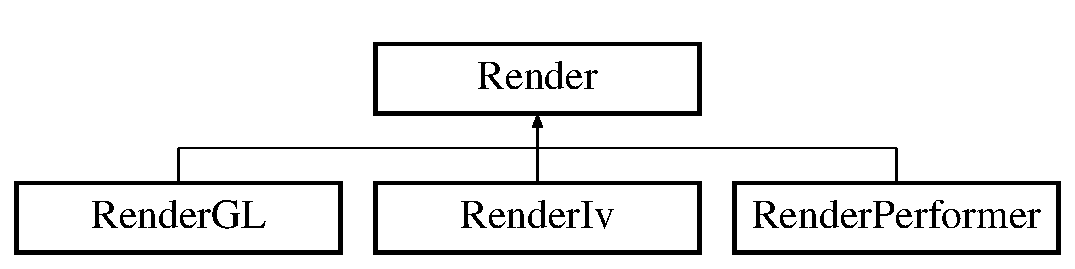
\includegraphics[height=2cm]{classRender}
\end{center}
\end{figure}
\subsection*{Public Methods}
\begin{CompactItemize}
\item 
{\bf Render} ()
\item 
{\bf Render} (string filepath)
\item 
{\bf Render} ({\bf Scene} $\ast$s, string filepath)
\item 
virtual {\bf $\sim$Render} ()
\item 
virtual void {\bf Init} ()
\begin{CompactList}\small\item\em Initialized the renderer.\item\end{CompactList}\item 
virtual void {\bf Handle\-Events} ()
\begin{CompactList}\small\item\em Process IO events.\item\end{CompactList}\item 
virtual void {\bf Main\-Loop} ({\bf Gui} $\ast$g)
\begin{CompactList}\small\item\em If Control\-Freak = true, then Main\-Loop is entered here.\item\end{CompactList}\item 
virtual void {\bf Reset} ()
\begin{CompactList}\small\item\em Reset the renderer.\item\end{CompactList}\item 
virtual void {\bf Terminate} ()
\begin{CompactList}\small\item\em Implement functions upon termination of the renderer.\item\end{CompactList}\item 
virtual void {\bf Set\-Frame\-List} ()
\begin{CompactList}\small\item\em Make the set of frames from State\-List and Time\-List.\item\end{CompactList}\item 
virtual void {\bf Make\-Animation\-Frames} (const list$<$ {\bf MSLVector} $>$ \&xlist, double deltat)
\begin{CompactList}\small\item\em Generate Frame\-List and set Animation\-Active to true.\item\end{CompactList}\item 
virtual void {\bf Make\-Animation\-Frames} (const list$<$ {\bf MSLVector} $>$ \&xlist, const list$<$ double $>$ \&timelist)
\item 
virtual void {\bf Draw\-Path} ()
\begin{CompactList}\small\item\em Display an entire path (the specific renderer determines how).\item\end{CompactList}\item 
virtual void {\bf Button\-Handle} (int b)
\begin{CompactList}\small\item\em Execute actions for render control window choices.\item\end{CompactList}\item 
void {\bf Set\-Scene} ({\bf Scene} $\ast$s)
\begin{CompactList}\small\item\em Change the associated scene.\item\end{CompactList}\end{CompactItemize}
\subsection*{Public Attributes}
\begin{CompactItemize}
\item 
string {\bf File\-Path}
\begin{CompactList}\small\item\em The path name for accessing files.\item\end{CompactList}\item 
list$<$ {\bf MSLVector} $>$ {\bf Frame\-List}
\begin{CompactList}\small\item\em The animation frames; each element is a Scene\-Configuration.\item\end{CompactList}\item 
double {\bf Frame\-Time}
\begin{CompactList}\small\item\em The amount of time for which a frame is shown.\item\end{CompactList}\item 
float {\bf Last\-Frame\-Time}
\begin{CompactList}\small\item\em The time stamp of the last frame change.\item\end{CompactList}\item 
float {\bf Frame\-Stuck\-Time}
\begin{CompactList}\small\item\em The amount of time since the last frame change.\item\end{CompactList}\item 
int {\bf Num\-Frames}
\begin{CompactList}\small\item\em The number of frames in the animation.\item\end{CompactList}\item 
double {\bf Animation\-Start\-Pause}
\begin{CompactList}\small\item\em Number of seconds to wait at the start of an animation.\item\end{CompactList}\item 
double {\bf Animation\-End\-Pause}
\begin{CompactList}\small\item\em Number of seconds to wait at the end of an animation.\item\end{CompactList}\item 
double {\bf Animation\-Time\-Scale}
\begin{CompactList}\small\item\em The speedup factor for the animation (1.0 = normal speed).\item\end{CompactList}\item 
double {\bf real\-Animation\-Time\-Scale}
\item 
double {\bf Animation\-Time\-Scale\_\-prev}
\item 
double {\bf real\-Animation\-Time\-Scale\_\-prev}
\item 
int {\bf Animation\-Frame\-Index}
\begin{CompactList}\small\item\em The index in Frame\-List of the frame that should be currently shown.\item\end{CompactList}\item 
{\bf MSLVector} {\bf Current\-Animation\-Frame}
\begin{CompactList}\small\item\em The frame that should be shown currently.\item\end{CompactList}\item 
bool {\bf Animation\-Active}
\begin{CompactList}\small\item\em Set to true to start the animation.\item\end{CompactList}\item 
bool {\bf Control\-Freak}
\begin{CompactList}\small\item\em Set to true if the renderer needs main loop control; otherwise, iterated polling of Handle\-Events will be performed automatically.\item\end{CompactList}\item 
bool {\bf Render\-Ctl\-Window\-On}
\begin{CompactList}\small\item\em Is teh rendering control window currently displayed?\item\end{CompactList}\item 
bool {\bf Attached\-Camera\-On}
\begin{CompactList}\small\item\em Set to true for the viewpoint to be attached to a body.\item\end{CompactList}\item 
bool {\bf Bounding\-Box\-On}
\begin{CompactList}\small\item\em Set to true to draw a bounding box using S-$>$Lower\-World and S-$>$Upper\-World.\item\end{CompactList}\item 
bool {\bf Multiple\-Views\-On}
\begin{CompactList}\small\item\em Set to true to show multiple views simultaneously.\item\end{CompactList}\item 
bool {\bf Show\-Path\-On}
\begin{CompactList}\small\item\em Set to true to show the entire path.\item\end{CompactList}\item 
double {\bf Ambient\-Light}
\begin{CompactList}\small\item\em A parameter that controls the amount of light.\item\end{CompactList}\end{CompactItemize}
\subsection*{Protected Methods}
\begin{CompactItemize}
\item 
virtual void {\bf Set\-Current\-Animation\-Frame} ()
\begin{CompactList}\small\item\em This uses the Frame\-List to return the Scene\-Configuration that is supposed to be shown at the present time.\item\end{CompactList}\item 
virtual void {\bf Show\-Current\-Animation\-Frame} ()
\begin{CompactList}\small\item\em Display the current animation frame in a rendering window.\item\end{CompactList}\end{CompactItemize}
\subsection*{Protected Attributes}
\begin{CompactItemize}
\item 
{\bf Scene} $\ast$ {\bf S}
\begin{CompactList}\small\item\em Allow information from a {\bf Scene} {\rm (p.\,\pageref{classScene})} to be accessed.\item\end{CompactList}\item 
list$<$ {\bf MSLVector} $>$ {\bf State\-List}
\begin{CompactList}\small\item\em A sequence of state to use for animation (should be generated by {\bf Gui} {\rm (p.\,\pageref{classGui})}).\item\end{CompactList}\item 
list$<$ double $>$ {\bf Time\-List}
\begin{CompactList}\small\item\em The time stamps for the state sequence.\item\end{CompactList}\item 
list$<$ string $>$ {\bf Env\-List}
\item 
list$<$ string $>$ {\bf Body\-List}
\item 
float {\bf RGBRed} [RENDERCOLORS]
\begin{CompactList}\small\item\em RGB color values.\item\end{CompactList}\item 
float {\bf RGBGreen} [RENDERCOLORS]
\item 
float {\bf RGBBlue} [RENDERCOLORS]
\end{CompactItemize}


\subsection{Detailed Description}
A rendering class that accepts commands from a {\bf Gui} {\rm (p.\,\pageref{classGui})}, and determines using specific graphics libraries how to draw the results on a screen.

This hierarchy of classes contains different implementations of graphical rendering requests. For example, when a graphical user interface (GUI) requests that the a solution path is animated, a method in a Render class displays the bodies in motion using configurations obtained from the {\bf Scene} {\rm (p.\,\pageref{classScene})} class. Each derived class in Render corresponds to a different graphics system. Presently, there are renderers for Open Inventor and Open GL. The flexibility provided by these classes enables easy extensions to be made for other graphics libraries and platforms, such as Open Inventor.

The rendering is expressed in terms of a {\bf Scene} {\rm (p.\,\pageref{classScene})}, in which the  scene configuration gives the configuration of a collection of Bodies in a static Environment. 



\subsection{Constructor \& Destructor Documentation}
\index{Render@{Render}!Render@{Render}}
\index{Render@{Render}!Render@{Render}}
\subsubsection{\setlength{\rightskip}{0pt plus 5cm}Render::Render ()}\label{classRender_a0}


\index{Render@{Render}!Render@{Render}}
\index{Render@{Render}!Render@{Render}}
\subsubsection{\setlength{\rightskip}{0pt plus 5cm}Render::Render (string {\em filepath})}\label{classRender_a1}


\index{Render@{Render}!Render@{Render}}
\index{Render@{Render}!Render@{Render}}
\subsubsection{\setlength{\rightskip}{0pt plus 5cm}Render::Render ({\bf Scene} $\ast$ {\em s}, string {\em filepath})}\label{classRender_a2}


\index{Render@{Render}!~Render@{$\sim$Render}}
\index{~Render@{$\sim$Render}!Render@{Render}}
\subsubsection{\setlength{\rightskip}{0pt plus 5cm}virtual Render::$\sim$Render ()\hspace{0.3cm}{\tt  [inline, virtual]}}\label{classRender_a3}




\subsection{Member Function Documentation}
\index{Render@{Render}!ButtonHandle@{ButtonHandle}}
\index{ButtonHandle@{ButtonHandle}!Render@{Render}}
\subsubsection{\setlength{\rightskip}{0pt plus 5cm}void Render::Button\-Handle (int {\em b})\hspace{0.3cm}{\tt  [virtual]}}\label{classRender_a13}


Execute actions for render control window choices.

\index{Render@{Render}!DrawPath@{DrawPath}}
\index{DrawPath@{DrawPath}!Render@{Render}}
\subsubsection{\setlength{\rightskip}{0pt plus 5cm}virtual void Render::Draw\-Path ()\hspace{0.3cm}{\tt  [inline, virtual]}}\label{classRender_a12}


Display an entire path (the specific renderer determines how).



Reimplemented in {\bf Render\-GL} {\rm (p.\,\pageref{classRenderGL_b11})}.\index{Render@{Render}!HandleEvents@{HandleEvents}}
\index{HandleEvents@{HandleEvents}!Render@{Render}}
\subsubsection{\setlength{\rightskip}{0pt plus 5cm}virtual void Render::Handle\-Events ()\hspace{0.3cm}{\tt  [inline, virtual]}}\label{classRender_a5}


Process IO events.



Reimplemented in {\bf Render\-Performer} {\rm (p.\,\pageref{classRenderPerformer_a5})}.\index{Render@{Render}!Init@{Init}}
\index{Init@{Init}!Render@{Render}}
\subsubsection{\setlength{\rightskip}{0pt plus 5cm}void Render::Init ()\hspace{0.3cm}{\tt  [virtual]}}\label{classRender_a4}


Initialized the renderer.



Reimplemented in {\bf Render\-GL} {\rm (p.\,\pageref{classRenderGL_a5})}.\index{Render@{Render}!MainLoop@{MainLoop}}
\index{MainLoop@{MainLoop}!Render@{Render}}
\subsubsection{\setlength{\rightskip}{0pt plus 5cm}void Render::Main\-Loop ({\bf Gui} $\ast$ {\em g})\hspace{0.3cm}{\tt  [virtual]}}\label{classRender_a6}


If Control\-Freak = true, then Main\-Loop is entered here.



Reimplemented in {\bf Render\-GL} {\rm (p.\,\pageref{classRenderGL_a6})}.\index{Render@{Render}!MakeAnimationFrames@{MakeAnimationFrames}}
\index{MakeAnimationFrames@{MakeAnimationFrames}!Render@{Render}}
\subsubsection{\setlength{\rightskip}{0pt plus 5cm}void Render::Make\-Animation\-Frames (const list$<$ {\bf MSLVector} $>$ \& {\em xlist}, const list$<$ double $>$ \& {\em timelist})\hspace{0.3cm}{\tt  [virtual]}}\label{classRender_a11}


\index{Render@{Render}!MakeAnimationFrames@{MakeAnimationFrames}}
\index{MakeAnimationFrames@{MakeAnimationFrames}!Render@{Render}}
\subsubsection{\setlength{\rightskip}{0pt plus 5cm}void Render::Make\-Animation\-Frames (const list$<$ {\bf MSLVector} $>$ \& {\em xlist}, double {\em deltat})\hspace{0.3cm}{\tt  [virtual]}}\label{classRender_a10}


Generate Frame\-List and set Animation\-Active to true.

\index{Render@{Render}!Reset@{Reset}}
\index{Reset@{Reset}!Render@{Render}}
\subsubsection{\setlength{\rightskip}{0pt plus 5cm}void Render::Reset ()\hspace{0.3cm}{\tt  [virtual]}}\label{classRender_a7}


Reset the renderer.



Reimplemented in {\bf Render\-GL} {\rm (p.\,\pageref{classRenderGL_a4})}.\index{Render@{Render}!SetCurrentAnimationFrame@{SetCurrentAnimationFrame}}
\index{SetCurrentAnimationFrame@{SetCurrentAnimationFrame}!Render@{Render}}
\subsubsection{\setlength{\rightskip}{0pt plus 5cm}void Render::Set\-Current\-Animation\-Frame ()\hspace{0.3cm}{\tt  [protected, virtual]}}\label{classRender_b0}


This uses the Frame\-List to return the Scene\-Configuration that is supposed to be shown at the present time.

\index{Render@{Render}!SetFrameList@{SetFrameList}}
\index{SetFrameList@{SetFrameList}!Render@{Render}}
\subsubsection{\setlength{\rightskip}{0pt plus 5cm}void Render::Set\-Frame\-List ()\hspace{0.3cm}{\tt  [virtual]}}\label{classRender_a9}


Make the set of frames from State\-List and Time\-List.

\index{Render@{Render}!SetScene@{SetScene}}
\index{SetScene@{SetScene}!Render@{Render}}
\subsubsection{\setlength{\rightskip}{0pt plus 5cm}void Render::Set\-Scene ({\bf Scene} $\ast$ {\em s})}\label{classRender_a14}


Change the associated scene.

\index{Render@{Render}!ShowCurrentAnimationFrame@{ShowCurrentAnimationFrame}}
\index{ShowCurrentAnimationFrame@{ShowCurrentAnimationFrame}!Render@{Render}}
\subsubsection{\setlength{\rightskip}{0pt plus 5cm}virtual void Render::Show\-Current\-Animation\-Frame ()\hspace{0.3cm}{\tt  [inline, protected, virtual]}}\label{classRender_b1}


Display the current animation frame in a rendering window.



Reimplemented in {\bf Render\-Performer} {\rm (p.\,\pageref{classRenderPerformer_b0})}.\index{Render@{Render}!Terminate@{Terminate}}
\index{Terminate@{Terminate}!Render@{Render}}
\subsubsection{\setlength{\rightskip}{0pt plus 5cm}virtual void Render::Terminate ()\hspace{0.3cm}{\tt  [inline, virtual]}}\label{classRender_a8}


Implement functions upon termination of the renderer.



Reimplemented in {\bf Render\-Performer} {\rm (p.\,\pageref{classRenderPerformer_a6})}.

\subsection{Member Data Documentation}
\index{Render@{Render}!AmbientLight@{AmbientLight}}
\index{AmbientLight@{AmbientLight}!Render@{Render}}
\subsubsection{\setlength{\rightskip}{0pt plus 5cm}double Render::Ambient\-Light}\label{classRender_m21}


A parameter that controls the amount of light.

\index{Render@{Render}!AnimationActive@{AnimationActive}}
\index{AnimationActive@{AnimationActive}!Render@{Render}}
\subsubsection{\setlength{\rightskip}{0pt plus 5cm}bool Render::Animation\-Active}\label{classRender_m14}


Set to true to start the animation.

\index{Render@{Render}!AnimationEndPause@{AnimationEndPause}}
\index{AnimationEndPause@{AnimationEndPause}!Render@{Render}}
\subsubsection{\setlength{\rightskip}{0pt plus 5cm}double Render::Animation\-End\-Pause}\label{classRender_m7}


Number of seconds to wait at the end of an animation.

\index{Render@{Render}!AnimationFrameIndex@{AnimationFrameIndex}}
\index{AnimationFrameIndex@{AnimationFrameIndex}!Render@{Render}}
\subsubsection{\setlength{\rightskip}{0pt plus 5cm}int Render::Animation\-Frame\-Index}\label{classRender_m12}


The index in Frame\-List of the frame that should be currently shown.

\index{Render@{Render}!AnimationStartPause@{AnimationStartPause}}
\index{AnimationStartPause@{AnimationStartPause}!Render@{Render}}
\subsubsection{\setlength{\rightskip}{0pt plus 5cm}double Render::Animation\-Start\-Pause}\label{classRender_m6}


Number of seconds to wait at the start of an animation.

\index{Render@{Render}!AnimationTimeScale@{AnimationTimeScale}}
\index{AnimationTimeScale@{AnimationTimeScale}!Render@{Render}}
\subsubsection{\setlength{\rightskip}{0pt plus 5cm}double Render::Animation\-Time\-Scale}\label{classRender_m8}


The speedup factor for the animation (1.0 = normal speed).

\index{Render@{Render}!AnimationTimeScale_prev@{AnimationTimeScale\_\-prev}}
\index{AnimationTimeScale_prev@{AnimationTimeScale\_\-prev}!Render@{Render}}
\subsubsection{\setlength{\rightskip}{0pt plus 5cm}double Render::Animation\-Time\-Scale\_\-prev}\label{classRender_m10}


\index{Render@{Render}!AttachedCameraOn@{AttachedCameraOn}}
\index{AttachedCameraOn@{AttachedCameraOn}!Render@{Render}}
\subsubsection{\setlength{\rightskip}{0pt plus 5cm}bool Render::Attached\-Camera\-On}\label{classRender_m17}


Set to true for the viewpoint to be attached to a body.

\index{Render@{Render}!BodyList@{BodyList}}
\index{BodyList@{BodyList}!Render@{Render}}
\subsubsection{\setlength{\rightskip}{0pt plus 5cm}list$<$string$>$ Render::Body\-List\hspace{0.3cm}{\tt  [protected]}}\label{classRender_n4}


\index{Render@{Render}!BoundingBoxOn@{BoundingBoxOn}}
\index{BoundingBoxOn@{BoundingBoxOn}!Render@{Render}}
\subsubsection{\setlength{\rightskip}{0pt plus 5cm}bool Render::Bounding\-Box\-On}\label{classRender_m18}


Set to true to draw a bounding box using S-$>$Lower\-World and S-$>$Upper\-World.

\index{Render@{Render}!ControlFreak@{ControlFreak}}
\index{ControlFreak@{ControlFreak}!Render@{Render}}
\subsubsection{\setlength{\rightskip}{0pt plus 5cm}bool Render::Control\-Freak}\label{classRender_m15}


Set to true if the renderer needs main loop control; otherwise, iterated polling of Handle\-Events will be performed automatically.

\index{Render@{Render}!CurrentAnimationFrame@{CurrentAnimationFrame}}
\index{CurrentAnimationFrame@{CurrentAnimationFrame}!Render@{Render}}
\subsubsection{\setlength{\rightskip}{0pt plus 5cm}{\bf MSLVector} Render::Current\-Animation\-Frame}\label{classRender_m13}


The frame that should be shown currently.

\index{Render@{Render}!EnvList@{EnvList}}
\index{EnvList@{EnvList}!Render@{Render}}
\subsubsection{\setlength{\rightskip}{0pt plus 5cm}list$<$string$>$ Render::Env\-List\hspace{0.3cm}{\tt  [protected]}}\label{classRender_n3}


\index{Render@{Render}!FilePath@{FilePath}}
\index{FilePath@{FilePath}!Render@{Render}}
\subsubsection{\setlength{\rightskip}{0pt plus 5cm}string Render::File\-Path}\label{classRender_m0}


The path name for accessing files.

\index{Render@{Render}!FrameList@{FrameList}}
\index{FrameList@{FrameList}!Render@{Render}}
\subsubsection{\setlength{\rightskip}{0pt plus 5cm}list$<${\bf MSLVector}$>$ Render::Frame\-List}\label{classRender_m1}


The animation frames; each element is a Scene\-Configuration.

\index{Render@{Render}!FrameStuckTime@{FrameStuckTime}}
\index{FrameStuckTime@{FrameStuckTime}!Render@{Render}}
\subsubsection{\setlength{\rightskip}{0pt plus 5cm}float Render::Frame\-Stuck\-Time}\label{classRender_m4}


The amount of time since the last frame change.

\index{Render@{Render}!FrameTime@{FrameTime}}
\index{FrameTime@{FrameTime}!Render@{Render}}
\subsubsection{\setlength{\rightskip}{0pt plus 5cm}double Render::Frame\-Time}\label{classRender_m2}


The amount of time for which a frame is shown.

\index{Render@{Render}!LastFrameTime@{LastFrameTime}}
\index{LastFrameTime@{LastFrameTime}!Render@{Render}}
\subsubsection{\setlength{\rightskip}{0pt plus 5cm}float Render::Last\-Frame\-Time}\label{classRender_m3}


The time stamp of the last frame change.

\index{Render@{Render}!MultipleViewsOn@{MultipleViewsOn}}
\index{MultipleViewsOn@{MultipleViewsOn}!Render@{Render}}
\subsubsection{\setlength{\rightskip}{0pt plus 5cm}bool Render::Multiple\-Views\-On}\label{classRender_m19}


Set to true to show multiple views simultaneously.

\index{Render@{Render}!NumFrames@{NumFrames}}
\index{NumFrames@{NumFrames}!Render@{Render}}
\subsubsection{\setlength{\rightskip}{0pt plus 5cm}int Render::Num\-Frames}\label{classRender_m5}


The number of frames in the animation.

\index{Render@{Render}!realAnimationTimeScale@{realAnimationTimeScale}}
\index{realAnimationTimeScale@{realAnimationTimeScale}!Render@{Render}}
\subsubsection{\setlength{\rightskip}{0pt plus 5cm}double Render::real\-Animation\-Time\-Scale}\label{classRender_m9}


\index{Render@{Render}!realAnimationTimeScale_prev@{realAnimationTimeScale\_\-prev}}
\index{realAnimationTimeScale_prev@{realAnimationTimeScale\_\-prev}!Render@{Render}}
\subsubsection{\setlength{\rightskip}{0pt plus 5cm}double Render::real\-Animation\-Time\-Scale\_\-prev}\label{classRender_m11}


\index{Render@{Render}!RenderCtlWindowOn@{RenderCtlWindowOn}}
\index{RenderCtlWindowOn@{RenderCtlWindowOn}!Render@{Render}}
\subsubsection{\setlength{\rightskip}{0pt plus 5cm}bool Render::Render\-Ctl\-Window\-On}\label{classRender_m16}


Is teh rendering control window currently displayed?

\index{Render@{Render}!RGBBlue@{RGBBlue}}
\index{RGBBlue@{RGBBlue}!Render@{Render}}
\subsubsection{\setlength{\rightskip}{0pt plus 5cm}float Render::RGBBlue[RENDERCOLORS]\hspace{0.3cm}{\tt  [protected]}}\label{classRender_n7}


\index{Render@{Render}!RGBGreen@{RGBGreen}}
\index{RGBGreen@{RGBGreen}!Render@{Render}}
\subsubsection{\setlength{\rightskip}{0pt plus 5cm}float Render::RGBGreen[RENDERCOLORS]\hspace{0.3cm}{\tt  [protected]}}\label{classRender_n6}


\index{Render@{Render}!RGBRed@{RGBRed}}
\index{RGBRed@{RGBRed}!Render@{Render}}
\subsubsection{\setlength{\rightskip}{0pt plus 5cm}float Render::RGBRed[RENDERCOLORS]\hspace{0.3cm}{\tt  [protected]}}\label{classRender_n5}


RGB color values.

\index{Render@{Render}!S@{S}}
\index{S@{S}!Render@{Render}}
\subsubsection{\setlength{\rightskip}{0pt plus 5cm}{\bf Scene}$\ast$ Render::S\hspace{0.3cm}{\tt  [protected]}}\label{classRender_n0}


Allow information from a {\bf Scene} {\rm (p.\,\pageref{classScene})} to be accessed.

\index{Render@{Render}!ShowPathOn@{ShowPathOn}}
\index{ShowPathOn@{ShowPathOn}!Render@{Render}}
\subsubsection{\setlength{\rightskip}{0pt plus 5cm}bool Render::Show\-Path\-On}\label{classRender_m20}


Set to true to show the entire path.

\index{Render@{Render}!StateList@{StateList}}
\index{StateList@{StateList}!Render@{Render}}
\subsubsection{\setlength{\rightskip}{0pt plus 5cm}list$<${\bf MSLVector}$>$ Render::State\-List\hspace{0.3cm}{\tt  [protected]}}\label{classRender_n1}


A sequence of state to use for animation (should be generated by {\bf Gui} {\rm (p.\,\pageref{classGui})}).

\index{Render@{Render}!TimeList@{TimeList}}
\index{TimeList@{TimeList}!Render@{Render}}
\subsubsection{\setlength{\rightskip}{0pt plus 5cm}list$<$double$>$ Render::Time\-List\hspace{0.3cm}{\tt  [protected]}}\label{classRender_n2}


The time stamps for the state sequence.



The documentation for this class was generated from the following files:\begin{CompactItemize}
\item 
{\bf render.h}\item 
{\bf render.C}\end{CompactItemize}
